\documentclass[11pt,pdftex,twocolumn]{article}
\usepackage{alltt}
\usepackage[dvips]{graphicx}
\usepackage{verbatim}
\usepackage[margin=1in, paperwidth=8.5in, paperheight=11in]{geometry}
\usepackage{url}

\title{NFS Trace Deconstruction: 
Server Side NFS Identification and Client-Side Packet Tracing in a Virtualized Environment}
\author{Rob Jellinek and Adam Vail}
\begin{document}
\maketitle

\begin{abstract}
This paper investigates server-side methods for determining whether NFS client are virtualized or native. We perform client-side and server-side network traces that identify two key differences that can be used as heuristics in identifying virtualized clients. First, virtualized clients using bridged networking can often be detected by the first three octets of their MAC address at the link layer, which are set to unique defaults by most common virtualization platforms. Second, virtualized clients using user-mode networking experience substantial latency in their network stack. Clients can then be distinguished according to bandwidth profiles. Finally, we investigate the sources of user-mode networking latency, and identify memory management in network address translation as the primary contributor to slowdown.
\end{abstract}

\section{Introduction}
This paper investigates approaches by which an NFS server can differentiate requests originating from native, non-virtualized machines from those originating from virtual machines. 
Ultimately, it is desirable for an NFS server to be able to identify and group all virtual machines resident on the same physical machine. Such identification and grouping would allow the server to coalesce its outgoing network traffic to the virtual machines, in essence performing VM-based redundancy elimination. This would lead to better NFS performance, and lower network utilization.

Our approach consisted of three parts. First, we searched through the NFS 4.0 RFC specification to find operations that could potentially differ in the VM or physical context, or otherwise uniquely mark the origin of the client machine. Second, we performed a number of client and server-side tcpdump traces on NFS 4.0 \texttt{mount} operations as well as file transfers, with the goal of isolating differences in the action of the NFS protocol in the virtual and physical settings. Finally, we timed NFS reads of varying sizes in the virtual and physical settings in order to determine if timing differences could be used to distinguish physical from virtual clients. 

We learned several things from these investigations. First, we were unable to differentiate any aspect of the NFS protocol in the virtual setting from its behavior in the physical setting at the application layer, either in our reading of the NFS 4.0 RFC or in our tcpdump traces. This is not surprising, as there is nothing that should inherently differ about the behavior of the application layer in a virtual machine. Thus, unless explicit signals are incorporated into the NFS protocol for the purpose of identifying a client as virtualized, nothing from the vanilla NFS protocol implementation seems to identify the platform of the client. 

However, we were able to establish two heuristics for identifying virtualized NFS clients. First, our network traces showed that although NFS application-layer semantics were indistinguishable, VM-based clients could be identified by a unique MAC address assigned by default to virtual NICs when the VM is using bridged networking. Second, our NFS read timings showed that virtualized clients using user-mode (NAT) networking experience a substantial drop in bandwidth compared to a native baseline. By profiling client accesses and establishing a baseline bandwidth, it is possible to use bandwidth profiles to identify a virtualized guest in a controlled environment.

The remainder of our work focused on determining why and how user-mode networking suffers such a dramatic slowdown compared to bridged networking. In particular, we trace and identify the key points in the code path of QEMU+KVM user-mode networking that cause this slowdown.

The rest of the paper is organized as follows. We introduce and compare user-mode and bridged networking (SubSection \ref{subsec:networkIntro}), which form the basis of our heuristics for differentiating clients by MAC address (SubSection \ref{subsec:macaddrs}) and bandwidth profiles (SubSection \ref{subsec:BWprofiles}). Finally, we end by examining the source of slowdown in user-mode networking in KVM+QEMU (Section \ref{sec:codepath}).


%******************************
[TODO: incorporate below]

Looking lower in the network stack, however, we found that the MAC addresses assigned to the virtual NICs of bridged connections took on default values under all the virtualization platforms we investigated, which would allow a server to distinguish the virtualization platform of VM-based client applications in these cases. We discuss our findings and the implications in more detail in Section \ref{sec:macaddrs} below. Finally, we found that NFS reads from a KVM+QEMU VM using NAT networking and virtio PCI paravirtualized network driver took an average of 72\% longer than reads from a native-hardware client, while NFS reads from a KVM+QEMU VM using bridged networking with the virtio driver took an average of 26\% longer than the client running on the same underlying native-hardware setup. Our experiment and tests are discussed below in Section \ref{sec:NFSTiming}. 
%******************************

\section{NFS}

\subsection{Experimental Setup}
\label{subsec:expSetup}
The traces and timing experiments discussed below were run on a simple two-node topology connected by a Cisco E-2000 gigabit router. The client was a Thinkpad T60 with a dual-core 1.83GHz Intel T2400 CPU, 2GB RAM, and an Intel 82573L gigabit NIC. The server was an AMD Opteron 148 operating at 1GHz, with 1GB of RAM and a gigabit on-motherboard NIC. The client and server both used ext4 as their primary filesystem, and the client KVM+QEMU guest VM used ext4 on an 8GB QCOW2 virtual disk. The client was running Ubuntu 12.04LTS natively and in its guest VMs, and the server was running CentOS 5.2.

The tcpdump traces we collected were executed with the flags \texttt{tcpdump -vvnnXSs 1536} in order to examine the full contents of each NFS packet exchanged between the client and server.

\subsection{User-mode/Bridged Networking}
\label{subsec:networkIntro}
Both of the heuristics we discuss below rely on key differences in network behavior and timing caused by the two main virtual networking configurations used by guest VMs. Guest VMs can be configured to run either user-mode, or bridged networking.

User-mode networking performs network address translation (NAT) behind the host, which isolates guest VMs from the outside network. That is, no entities outside the physical host's network can see the guest VMs, and so without incorporating port-forwarding, those guests cannot be contacted from the outside. Importantly, this also has the effect that all guest VMs share a common IP and MAC address with the host; when the guest has an established TCP session open and the host receives packets destined for that guest, the host demultiplexes those packets and forwards them to the correct guest. 

KVM+QEMU uses the SLiRP protocol to perform network address translation. SLiRP was originally used to emulate TCP/IP and provide transport-layer functionality for users with dialup connections. The emulation code has been incorporated into the main branch of KVM+QEMU, and uses this emulation support to provide support for user-mode networking.

Bridged networking, on the other hand, uses a TAP device that is configured on the host. Both the physical NIC and the TAP device must be connected to a virtual network bridge on the host, which requires root access. Guest VMs then attach to the TAP device through their virtual interfaces and participate as full fledged members of the network. This means that their virtual NICs are assigned unique IP addresses that are visible to the outside network, as well as MAC addresses that must be unique within the network.


\subsection{Identifying Bridged Hosts by MAC Address}
\label{subsec:macaddrs}
While we did not discover characteristics of NFS application-layer requests or responses that indicate whether an NFS client is running on a VM or native hardware, we did find a distinguishing characteristic at layer 2 of virtualized clients' bridged networking stack. In virtual bridged networking, the guest network stack gets its own IP address and MAC address and appears as a separate host on the network, though it uses its host's physical NIC by passing packets through a tap device on the host (see SubSection \ref{subsec:bridgeVsNAT} below for details on bridging). The key thing to note is that the main virtualization platforms assign a default MAC address to the virtual NIC, which is then visible to the server in the MAC address fields of the Ethernet headers exchanged with the client. See Table \ref{tab:macaddrs} for a list of default MAC addresses assigned to virtual NICs in common virtualization platforms. 

This helps us distinguish virtual from native clients to some extent, but still leaves a lot to be desired if we wish to identify and group VM-based NFS clients. First, in the bridged context, it is possible for a client VM user to specify their MAC address to be anything they desire. These defaults are merely that: default settings allocated by the virtualization manager or hypervisor if the VM administrator does not specify an alternative address. So there is certainly a chance for false negatives, where virtual machines using bridging on a certain platform cannot be identified by their MAC address because the default MAC address is not used. Second, the identification is overly broad: the NFS server can detect that it is talking with a KVM+QEMU or VMWare guest VM, but it is not possible to identify those guest VMs as belonging to any given physical machine based on this information alone. 

\begin{center}
\begin{table*}[!ht]
		\center
		\begin{tabular}{|l|l|}
		\hline
			Virtualization Platform & MAC \\
		\hline
		\hline
			KVM+QEMU & 52:54:00 \\
			VMware ESX 3, Server, Workstation, Player	& 00-50-56, 00-0C-29, 00-05-69 \\
			Microsoft Hyper-V, Virtual Server, Virtual PC	& 00-03-FF \\
			Parallells Desktop, Workstation, Server, Virtuozzo & 00-1C-42 \\
			Virtual Iron 4 & 00-0F-4B \\
			Red Hat Xen	& 00-16-3E \\
			Oracle VM	& 00-16-3E \\
			XenSource	& 00-16-3E \\
			Novell Xen & 00-16-3E \\
			Sun xVM VirtualBox & 08-00-27 \\
		\hline
		\end{tabular}
	\caption{First three octets of default MAC addresses by virtualization platform\footnote{ \emph{(Source:http://www.techrepublic.com/blog/networking/mac-address-scorecard-for-common-virtual-machine-platforms/538)}}}
	\label{tab:macaddrs}
\end{table*}
\end{center}

\subsection{Identifying NATed Host by Bandwidth Profiles}
\label{subsec:BWprofiles}	

\begin{figure}
	\center
		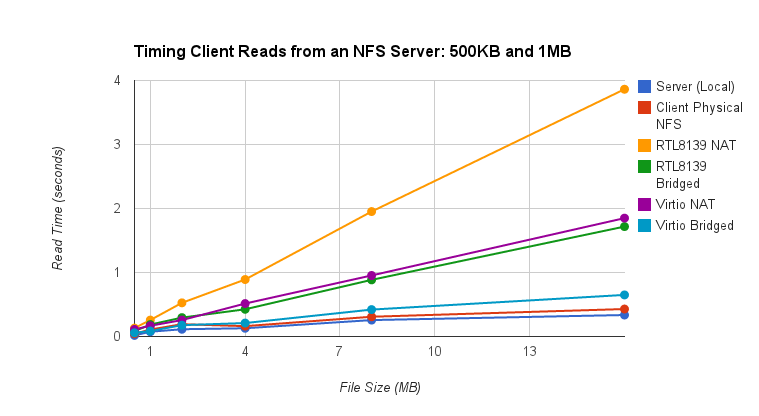
\includegraphics[scale=0.34]{timing_small.png}
	\caption{When reading small files, bandwidth profiles are not yet clearly ordered.}
	\label{fig:timing_small}
\end{figure}

\begin{figure}
	\center
		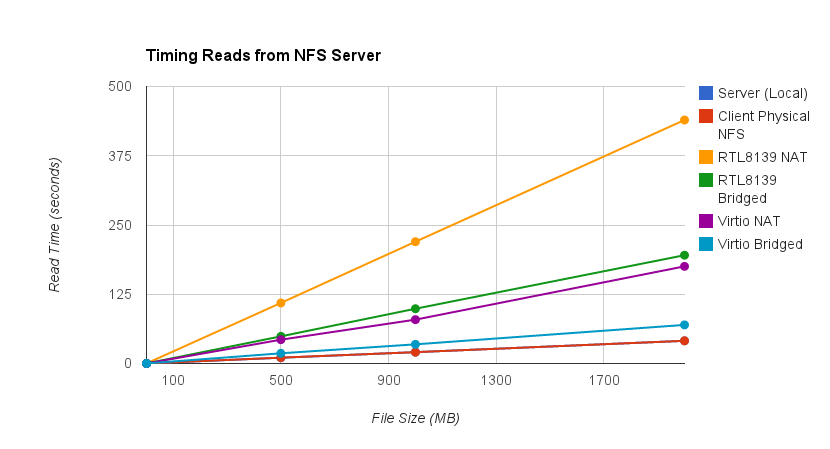
\includegraphics[scale=0.3]{timing_large.png}
	\caption{When reading larger files, the bandwidth profiles are clearly differentiated.}
	\label{fig:timing_large}
\end{figure}

The MAC address distinction does not help us in the case of VM-based clients that are using user-mode (NAT-based) networking instead of bridging, as NATed guests are not visible to the rest of the network and do not have an externally identifiable IP and MAC address. As discussed above, all guest VM traffic is rewritten inside the host to contain the MAC and IP addresses of the host NIC. However, user-mode networking suffers from a substantial slowdown compared to physical or bridged hosts. In a controlled environment, this dramtically decreased bandwidth relative to a native-client baseline can enable a server to conclude that the client is virtualized. 

%TODO: insert timing_small with additional file-size data points, and discuss them here. When does the relative BW ordering become stable?
Figures \ref{fig:timing_small} and \ref{fig:timing_large} show the results of timing tests in which the client VMs under various networking configurations read 500KB, 1MB, 500MB, 1GB, and 2GB files from an NFS server according to the configuration describe in Subsection \ref{subsec:expSetup}. Files were read in 4KB blocks, and file buffer caches were cleared between tests by running \texttt{echo 3 > /proc/sys/vm/drop\_caches}. Figure \ref{fig:timing_small} shows that when reading smaller files, the bandwidths of the various client-VM networking configurations have not yet achieved a stable relative ordering. However, when reading larger files, as shown in Figure \ref{fig:timing_large}, a clear relative bandwidth ordering emerges.

Not surprisingly, reads on the server itself (directly from the local ext4 file system) were fastest and were mirrored almost exactly by reads from the NFS client running on native hardware. Note that the reads performed locally on the server and from the native client differed by only 43 milliseconds across all tests, so their lines are coincident in Figure \ref{fig:timing_large}. Of the virtualized clients, using the paravirtualized virtio driver under bridged networking imposed only a slight overhead relative to the native-client baseline. However, switching to either the fully emulated RealTek RTL8139 virtual network driver or using NATed instead of bridged networking imposed a substantial bandwidth penalty. Doing both (using the RTL8139 under user-mode networking) results in 10.7x slowdown relative to our baseline. 

We can use this to our advantage in determining whether a client is physical or virtualized. In particular, we can break the configurations into bandwidth classes as shown in Table \ref{tab:NFSBandwidthProfiles}. The bandwidth profiles are sufficiently differentiated to allow the NFS server to use them to ``fingerprint'' incoming client connections after performing a sustained read to get an accurate bandwidth measure. While we emphasize that this is a heuristic and is not a foolproof means of identifying virtualized clients, when used in a controlled environment and in conjunction with the MAC-address profiling described in Subsection \ref{subsec:macaddrs}, an NFS server should be able to differentiate native clients from virtualized ones in many environments. 

\begin{table*}[htbp]
	\centering
		\begin{tabular}{|l|l|}
			\hline
			\textbf{Client Network Stack} & \textbf{Bandwidth} (MB/sec) \\
			\hline
			Native & 48.3 \\
			Virtio Bridged & 28.3 \\
			Virtio NAT & 11.9 \\
			RealTek Bridged & 10.2 \\
			RealTek NAT & 4.6 \\
			\hline
		\end{tabular}
	\caption{NFS Bandwidth Profiles}
	\label{tab:NFSBandwidthProfiles}
\end{table*}

\section{Following the Code Path}
\label{sec:codepath}
In order to determine where the bottlenecks are occurring using the RTL8139 driver which performs full emulation, we traced the code path of a packet from the guest's application layer through the guest and host network stacks. We provide an explanation of the traces and relevant functions for the code path for the transmit side below, and an outline of the path for the receive side in the Appendix, along with the code path followed by packets on the transmit side that are shared by both the NAT and bridged code. 


\subsection{RealTek 8139 NAT: Guest Transmit}
User-mode networking under QEMU uses network address translation (NAT) in order to allow a guest VM to establish connections with outside networks. QEMU performs address translation using a protocol from the 1990s known as SLiRP, which was originally used to provide TCP/IP access to dial-up shell account users by emulating the TCP/IP stack. Though that usage is largely obsolete, the same address translation techniques are applied in QEMU user-mode networking 

%\begin{verbatim}
%slirp_input:
%|          |
%|           -> m_get (allocates buffer space for packet to be copied into)
%|               |
%|                -> slirp_insque (manages doubly linked list of buffer space that is being used for the packets)
%|
% ->ip_input (converts ip fields to host representation using ntohs, manipulating buffer space that was created in m_get)
%    |
%    |
%     -> tcp_input (converts tcp fields to host format. Rewrites all the fields to host representation)
%         |
%         |
%          -> tcp_output (standard tcp things happen here. e.g. calculating receive window. There is a lot going on here. Flips tcp fields back from host byte order to network byte order)
%              |
%              |
%               -> ip_output (flips ip fields back to network byte order from host byte order)
%                   |
%                   |
%                    -> if_output 
%                        |     + Figures out which queue to place the packet on
%                        |         + fastq: meant for packets associated with interactive activities. Determined through the IPTOS_NODELAY flag set in the ip header of the packet
%                        |         + batchq: queue for non-interactive actions. This is a more efficient queue.
%                        |     + Favorite comment:
%                        |           "These are arbitrary numbers, probably not optimal"
%                        |     + creates a new doubly linked list through m_get, not entirely clear why they need it, it looks like another packet queue
%                        |
%                         -> if_start
%                             |    + Drains the fastq before the batchq
%                             |    + cleans up the buffers and frees memory after if_encap returns
%                             |      (i.e., it calls slirp_remque and m_free, which cleans up the buffers)
%                             |
%                              -> if_encap
%                                  |    + Copies packet headers into appropriate header structs, essentially preparing the packet
%                                  |
%                                   -> slirp_output
%                                       |         + Add slirp state info and pass the packet off to qemu to get it out to the wire
%                                       |
%                                        -> qemu_send_packet
%                                                       + Passes packet through several wrapper functions which finally ends with qemu_net_queue_append which adds the packet to a queue which I assume puts it on the wire.
%                                                        + wrapper for qemu_send_packet_async with the last argument set to NULL
%
%
%\end{verbatim}

\subsection{RealTek 8139 Bridged: Guest Transmit}
We first come out the end of the shared code (see Appendix) and get to tap_receive. The flow continues as follows:

tap_receive
tap_receive_raw
tap_write_packet
writev 


%\input{implementation}
%\input{evaluation}
%\input{future}
%\input{related}
%\input{conclusion}

\section{Appendix}

[TODO: provide a graph of the code that happens whether you're shared or bridged on a guest transmit]
The code is implementing a deisgn pattern through the following functions: 

GUEST NETWORK STACK finishes here
--- start QEMU user space emulating physical NIC here ---
rtl8139_transfer_frame 
qemu_send_packet
qemu_send_packet_async
qemu_send_packet_async_with_flags
qemu_net_queue_send
qemu_net_queue_deliver
qemu_deliver_packet
net_hub_port_receive
net_hub_receive
qemu_send_packet' (now it's running through different interfaces: figured out that it needs to be moving toward the TAP device.)
qemu_send_packet_async'
qemu_send_packet_async_with_flags'
qemu_net_queue_deliver'
qemu_deliver_packet'
tap_receive / net_slirp_receive -> slirp_input depending on whether you're using bridged or NAT.

This is shared by everyone. It's connecting the driver at the top to the actual networking at the bottom. 

------

RECEIVE SIDE:
These functions bridge the gap between the top of the host network stack and pass the incoming packets to the bottom of the guest network stack--the RTL8139 emulated network driver. 

\header{Bridged}
Here tap_send, etc., don't mess with the packet headers at all--they just pass the packets straight up to the guest from the physical interface, possibly via queue using qemu_notify--so the packets have come directly from the physical NIC and don't need to have their headers retranslated.

main_loop_wait
qemu_io_handler_poll
tap_send
tap_read_packet
if the size read > 0:
	qemu_send_packet_async
... continue to shared code. The interested reader can check out the KVM source, wazzup.

\header{NAT}
Everything is in host byte order, because it's passed through the full host network stack and is coming off the application layer of the host network stack. So at this stage everything gets ripped off and translated back to network byte order and passed to the RTL8139 network driver of the guest stack, which the once again decapsulates the packets for the guest application layer. So the flow is: decapsulate in host network stack; re-encapsulate here and pass to bottom of guest network stack; guest network stack re-decapsulates packet (essentially repeating the work of the host network stack, but with the headers that were modified by NATing). 

main_loop_wait
slirp_select_poll
tcp_output -- strips the headers
ip_output -- gets new headers based 
if_output
if_start
if_encap
slirp_output

This could be why we're getting weird iperf data--because 








{\footnotesize \bibliographystyle{acm}
\bibliography{references}}



\end{document}
